\section{Date: 2026-09-21}
\noindent \textbf{Series ID: PCU221122221122421} 

\noindent This series is titled Producer Price Index by Industry: Electric Power Distribution: Commercial Electric Power for New England Census Division and has a frequency of Monthly. The units are Index Dec 1990=100 and the seasonal adjustment is Not Seasonally Adjusted.The observation start date is 1971-01-01 and the observation end date is 2026-08-01.The popularity of this series is 1. \\ 

\noindent \textbf{Series ID: SYSIILPIBLEND} 

\noindent This series is titled Medical Services Expenditures by Disease: Symptoms; Signs; and Ill-Defined Conditions Price Index, Blended Account Basis and has a frequency of Annual. The units are Index 2017=100 and the seasonal adjustment is Not Seasonally Adjusted.The observation start date is 2000-01-01 and the observation end date is 2021-01-01.The popularity of this series is 1. \\ 

\subsection{Raw Regression}
\noindent Regresses the two series against each other directly. A significant result here can come just as easily from both series sharing a long-run trend as from any real relationship.

\begin{center}
\begin{tabular}{lclc}
\toprule
\textbf{Dep. Variable:}                  & value\_fred\_SYSIILPIBLEND & \textbf{  R-squared:         } &     0.933   \\
\textbf{Model:}                          &            OLS             & \textbf{  Adj. R-squared:    } &     0.929   \\
\textbf{Method:}                         &       Least Squares        & \textbf{  F-statistic:       } &     277.7   \\
\textbf{Date:}                           &      Mon, 21 Sep 2026      & \textbf{  Prob (F-statistic):} &  3.41e-13   \\
\textbf{Time:}                           &          17:16:08          & \textbf{  Log-Likelihood:    } &   -68.300   \\
\textbf{No. Observations:}               &               22           & \textbf{  AIC:               } &     140.6   \\
\textbf{Df Residuals:}                   &               20           & \textbf{  BIC:               } &     142.8   \\
\textbf{Df Model:}                       &                1           & \textbf{                     } &             \\
\textbf{Covariance Type:}                &         nonrobust          & \textbf{                     } &             \\
\bottomrule
\end{tabular}
\begin{tabular}{lcccccc}
                                         & \textbf{coef} & \textbf{std err} & \textbf{t} & \textbf{P$> |$t$|$} & \textbf{[0.025} & \textbf{0.975]}  \\
\midrule
\textbf{const}                           &      -6.0876  &        5.281     &    -1.153  &         0.263        &      -17.103    &        4.928     \\
\textbf{value\_fred\_PCU221122221122421} &       0.5458  &        0.033     &    16.664  &         0.000        &        0.477    &        0.614     \\
\bottomrule
\end{tabular}
\begin{tabular}{lclc}
\textbf{Omnibus:}       &  6.881 & \textbf{  Durbin-Watson:     } &    1.268  \\
\textbf{Prob(Omnibus):} &  0.032 & \textbf{  Jarque-Bera (JB):  } &    5.911  \\
\textbf{Skew:}          &  0.534 & \textbf{  Prob(JB):          } &   0.0521  \\
\textbf{Kurtosis:}      &  5.304 & \textbf{  Cond. No.          } &     706.  \\
\bottomrule
\end{tabular}
%\caption{OLS Regression Results}
\end{center}

Notes: \newline
 [1] Standard Errors assume that the covariance matrix of the errors is correctly specified.

\begin{figure}
\centering
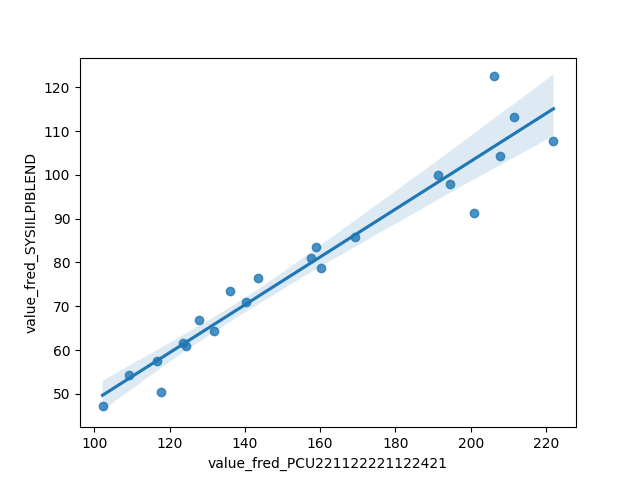
\includegraphics[scale = 0.9]{plots/plot_2026-09-21.png}
\caption{Raw Regression Plot for 2026-09-21}
\end{figure}
\newpage
\subsection{Detrended Regression}
\noindent Regresses the residuals of each series after removing its own linear time trend, so a shared trend can no longer drive the result on its own. A relationship that stays significant here is better evidence of a genuine link between the two series.

\begin{center}
\begin{tabular}{lclc}
\toprule
\textbf{Dep. Variable:}                             & value\_fred\_SYSIILPIBLEND\_detrended & \textbf{  R-squared:         } &     0.022   \\
\textbf{Model:}                                     &                  OLS                  & \textbf{  Adj. R-squared:    } &    -0.027   \\
\textbf{Method:}                                    &             Least Squares             & \textbf{  F-statistic:       } &    0.4428   \\
\textbf{Date:}                                      &            Mon, 21 Sep 2026           & \textbf{  Prob (F-statistic):} &    0.513    \\
\textbf{Time:}                                      &                17:16:08               & \textbf{  Log-Likelihood:    } &   -54.441   \\
\textbf{No. Observations:}                          &                     22                & \textbf{  AIC:               } &     112.9   \\
\textbf{Df Residuals:}                              &                     20                & \textbf{  BIC:               } &     115.1   \\
\textbf{Df Model:}                                  &                      1                & \textbf{                     } &             \\
\textbf{Covariance Type:}                           &               nonrobust               & \textbf{                     } &             \\
\bottomrule
\end{tabular}
\begin{tabular}{lcccccc}
                                                    & \textbf{coef} & \textbf{std err} & \textbf{t} & \textbf{P$> |$t$|$} & \textbf{[0.025} & \textbf{0.975]}  \\
\midrule
\textbf{const}                                      &    4.119e-14  &        0.643     &  6.41e-14  &         1.000        &       -1.340    &        1.340     \\
\textbf{value\_fred\_PCU221122221122421\_detrended} &       0.0480  &        0.072     &     0.665  &         0.513        &       -0.103    &        0.199     \\
\bottomrule
\end{tabular}
\begin{tabular}{lclc}
\textbf{Omnibus:}       & 12.738 & \textbf{  Durbin-Watson:     } &    0.457  \\
\textbf{Prob(Omnibus):} &  0.002 & \textbf{  Jarque-Bera (JB):  } &   12.678  \\
\textbf{Skew:}          &  1.200 & \textbf{  Prob(JB):          } &  0.00177  \\
\textbf{Kurtosis:}      &  5.841 & \textbf{  Cond. No.          } &     8.90  \\
\bottomrule
\end{tabular}
%\caption{OLS Regression Results}
\end{center}

Notes: \newline
 [1] Standard Errors assume that the covariance matrix of the errors is correctly specified.

\begin{figure}
\centering
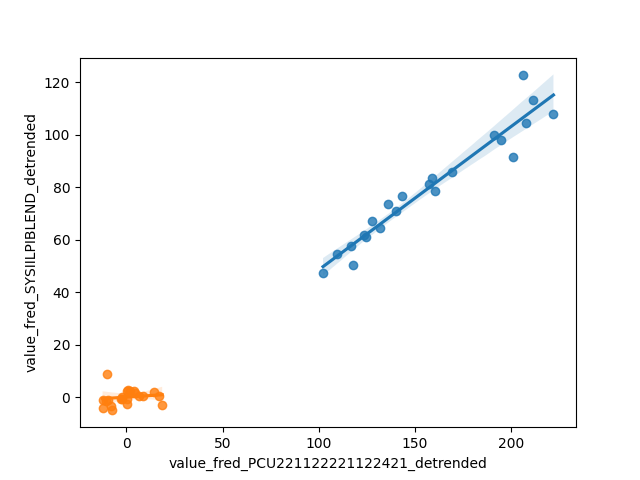
\includegraphics[scale = 0.9]{plots/plot_2026-09-21_detrended.png}
\caption{Detrended Regression Plot for 2026-09-21}
\end{figure}
\newpage
